\subsection{Distributed Memory Model}
\sciwms{} stores the data topology locally and fetches numerical
attributes hosted externally from the federation as needed for
rendering. Given a request for the visualization of a attributes
pertaining to a region of interest, the visualization pipeline
consists of first computing the sample locations withing the region of
interest, using the implicit representation for \cgrid{} and \rtree{}
for \ugrid{} topologies, then fetching the external attributes via
\ogc{} web-services. For rendering, the sample connectivity within the
area of interest is constructed from the connectivity array which is
used for interpolation.

The local topology cache and external attribute mechanism defines a
distributed memory model for datasets registered with \sciwms{} as
visualized in figure~\ref{fig:sciwms_mem_model}. The grid on the left,
depicts a regular grid stored locally to \sciwms{}. A possible region
of interest is highlighted by the red-dashed square. Attributes are
stored externally by federations members and are exposed to \sciwms{}
in such a way as it can be visualized using the table on the left of
the figure. Different attribute layers are represented by the rows of
the table while columns correspond to memory locations of attribute
values associated with the topology. The region of interest may correspond
to memory locations highlighted by the red cells in the table. Given
the request for a rendering of an attribute layer(s), \sciwms{}
dispatches a request for externally hosted numerical data necessary to
render the region of interest. 
\begin{figure}[ht!]
  \centering
  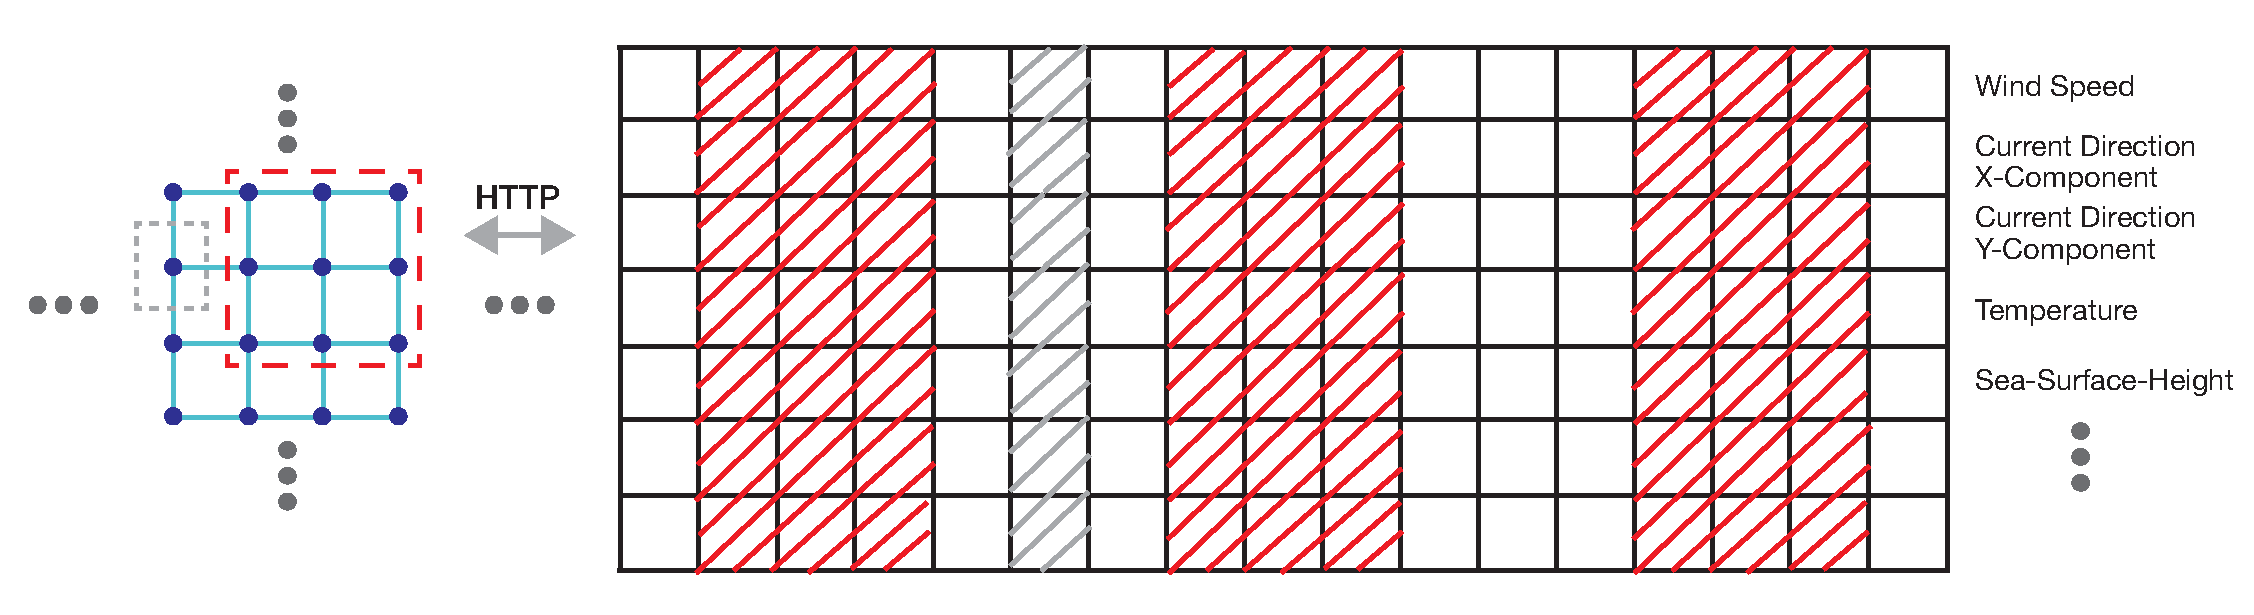
\includegraphics[width=\textwidth]{../figs/topology_memModel}
  \caption{\sciwms{} distributed memory model. The grid on the left
    shows a regular grid stored locally to the \sciwms{} server and
    the table to the right visualizes the attribute memory locations
    hosted by an external web-service. While attributes may be
    heterogeneous, the external attribute table offers a convenient
    first order conceptualization. The relationship between topology
    and attributes is specified through \ncml{} meta data.}
  \label{fig:sciwms_mem_model}
\end{figure}
